\documentclass[11pt,a4paper]{article}

% ============================================================
% Paper 25 -- Variational Foundation of Bottom-Up Quantum Gravity
% ============================================================

\usepackage[utf8]{inputenc}
\usepackage[T1]{fontenc}
\usepackage{lmodern}
\usepackage[a4paper,margin=2.6cm]{geometry}
\usepackage{amsmath,amssymb,amsfonts,bm}
\usepackage{mathtools}
\usepackage{booktabs}
\usepackage{array}
\usepackage{longtable}      % ajouté
\usepackage{graphicx}       % ajouté
\usepackage{hyperref}
\usepackage{xcolor}

\hypersetup{
  colorlinks=true,
  linkcolor=blue!60!black,
  citecolor=blue!60!black,
  urlcolor=blue!60!black
}

\newcommand{\Lent}{L_{\rm ent}}
\newcommand{\He}{\mathcal H}
\newcommand{\alphEff}{\alpha_{\rm eff}}

\title{\textbf{Paper 25 --- Variational Foundation of Bottom-Up Quantum Gravity}\\[0.35em]
\large From Entanglement Equilibrium to Effective Einstein Equations}

\author{Farid Hamdad\\
\small Bottom-Up Quantum Gravity Program}

\date{2026}

\begin{document}

\maketitle

\begin{abstract}
Bottom-Up Quantum Gravity (BuP) is reformulated as a variational theory of
entanglement equilibrium. The fundamental object is not a smooth metric, but a
finite mutual-information graph
\[
  W_{ij}=I(i:j),
\]
from which one constructs the entanglement Laplacian
\[
  L_{\rm ent}=D-W.
\]
The central dynamical condition is the discrete variational equilibrium equation
\[
  \frac{\delta S_{\rm BuP}[W,\rho]}{\delta W_{ij}}=0.
\]
This paper assembles the main theoretical and numerical branches of the BuP
program into a single foundation: the weak-field entanglement Green function,
the effective propagator law, the cosmological dimensional sector, the galactic
SPARC sector, the spectral continuum limit, the Ollivier--Ricci curvature
limit, the modular source sector, the effective Einstein equation, the
correction tensor, the SLACS fixed point, the gravitational-wave sector, and
the modular tomography proposal. The resulting continuum target is
\[
G_{\mu\nu}[g^{\rm ent}]
+\Lambda_{\rm ent}g_{\mu\nu}^{\rm ent}
=
8\pi G_{\rm eff}T_{\mu\nu}^{\rm ent}
+\mathcal H_{\mu\nu}^{\rm BuP}.
\]
The claim is not that a complete theorem has already been proven, but that BuP
now possesses a coherent variational chain from entanglement graphs to
effective Einstein dynamics, with clearly identified analytical debts.
\end{abstract}

\tableofcontents

\section{Introduction}

The usual formulation of gravity takes the metric tensor \(g_{\mu\nu}\) as the
fundamental geometric field. Bottom-Up Quantum Gravity reverses this order. It
starts from quantum information and asks whether geometry, matter,
gravitational potentials, and Einstein-like dynamics can emerge from a finite
quantum correlation structure.

The fundamental variable is the mutual-information graph
\begin{equation}
  W_{ij}=I(i:j),
\end{equation}
where \(I(i:j)\) denotes the mutual information between the microscopic degrees
of freedom \(i\) and \(j\). From \(W\), one constructs the graph degree matrix
\begin{equation}
  D_{ii}=\sum_j W_{ij},
\end{equation}
and the entanglement Laplacian
\begin{equation}
  L_{\rm ent}=D-W.
\end{equation}

The central proposal of this paper is that BuP should be regarded as a
variational theory of entanglement equilibrium. The discrete equilibrium
equation is
\begin{equation}
  \boxed{
  \frac{\delta S_{\rm BuP}[W,\rho]}{\delta W_{ij}}=0.
  }
  \label{eq:fundamental_equilibrium}
\end{equation}
Its smooth local continuum target is
\begin{equation}
  \boxed{
  G_{\mu\nu}[g^{\rm ent}]
  +
  \Lambda_{\rm ent}g_{\mu\nu}^{\rm ent}
  =
  8\pi G_{\rm eff}T_{\mu\nu}^{\rm ent}
  +
  \mathcal H_{\mu\nu}^{\rm BuP}.
  }
  \label{eq:effective_einstein_target}
\end{equation}

Here \(g_{\mu\nu}^{\rm ent}\) is an emergent entanglement metric,
\(T_{\mu\nu}^{\rm ent}\) is an emergent modular stress-energy tensor,
\(\Lambda_{\rm ent}\) is an entanglement cosmological term, \(G_{\rm eff}\) is
an effective gravitational coupling, and \(\mathcal H_{\mu\nu}^{\rm BuP}\)
collects finite-size, spectral, curvature, source, dimensional, nonlocal,
topological, and dynamical corrections.

The purpose of Paper 25 is to assemble the preceding BuP papers into a single
mathematical architecture. The key message is:
\begin{equation}
  \boxed{
  \text{BuP is a variational theory of entanglement equilibrium whose smooth
  local limit is an effective Einstein equation.}
  }
\end{equation}

% --- FIGURE 1 : Variational chain ---------------------------------------------
\begin{figure}[htbp]
\centering
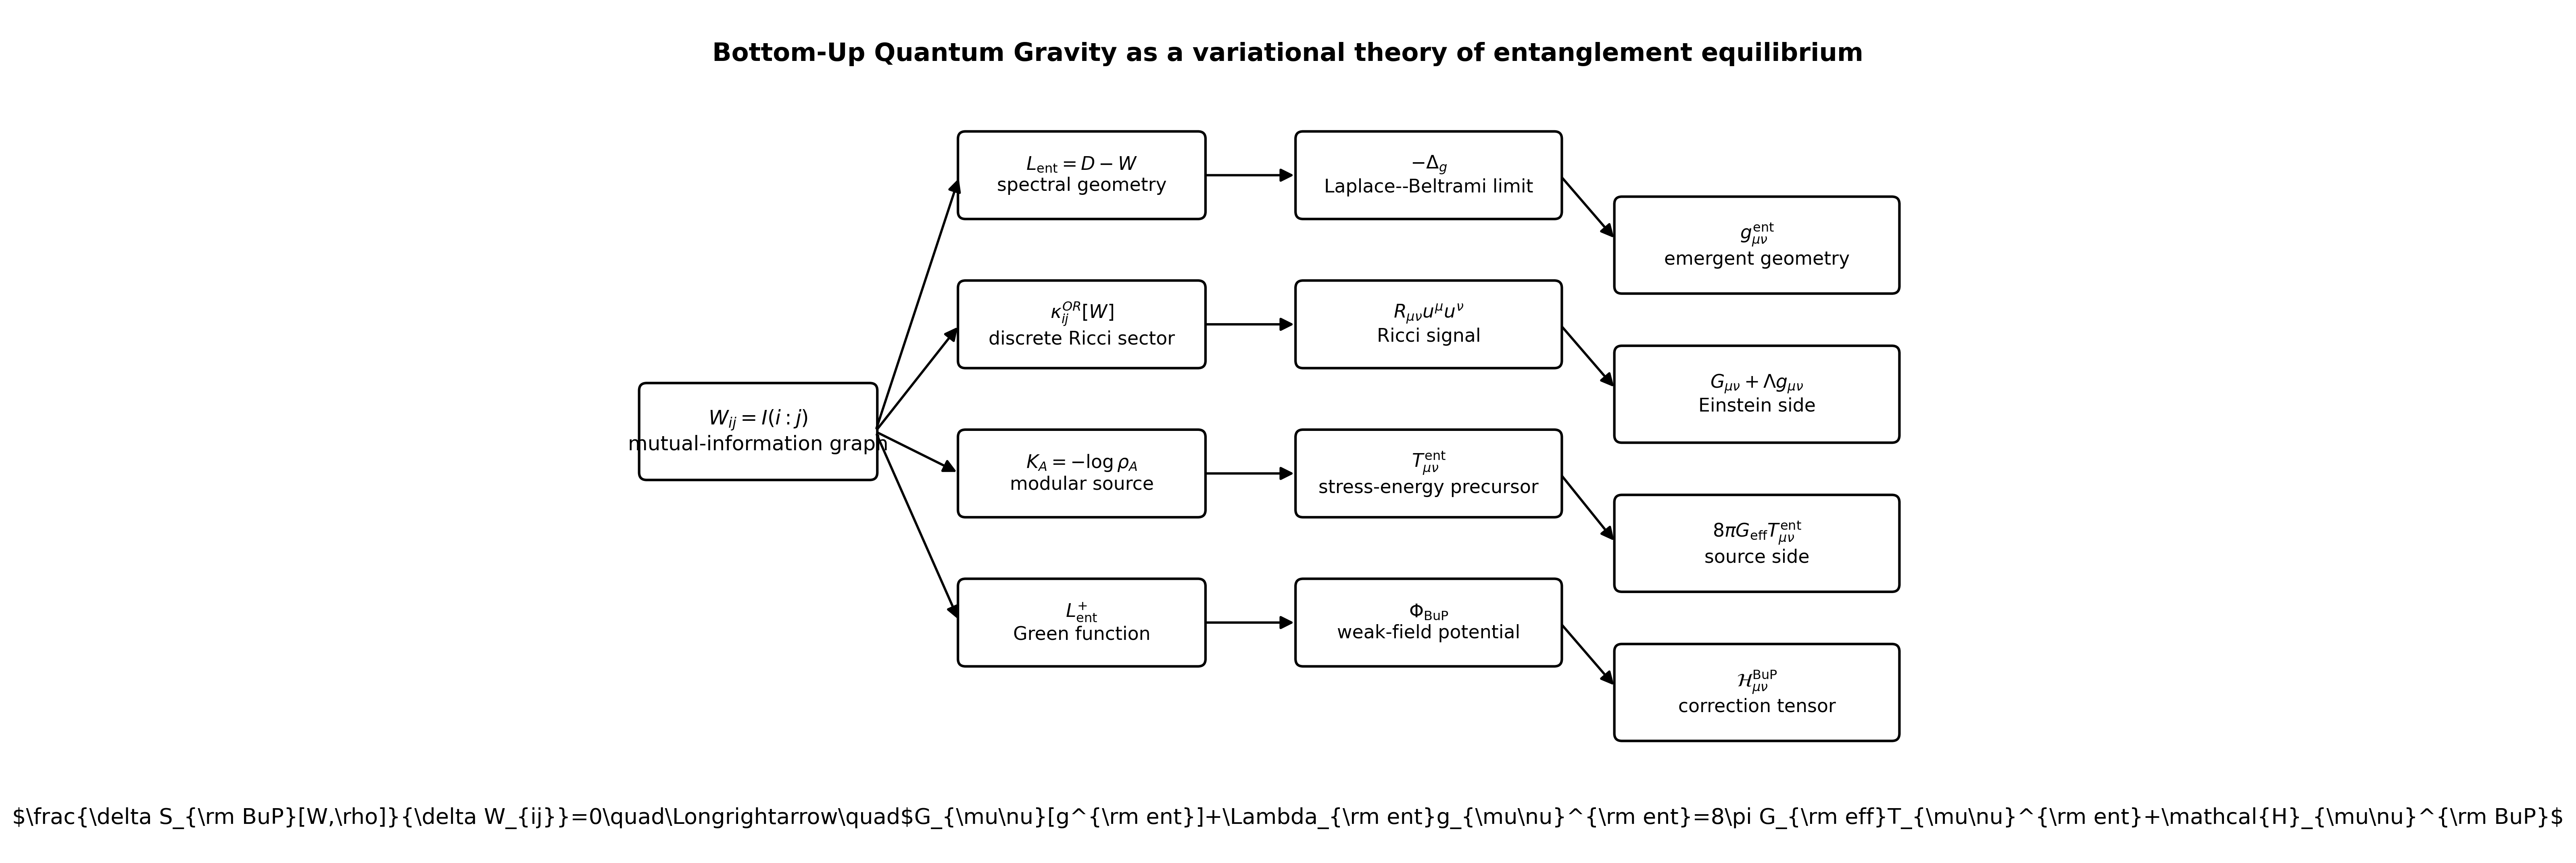
\includegraphics[width=\textwidth]{figures/fig01_variational_chain.png}
\caption{
Variational chain of Bottom-Up Quantum Gravity. The fundamental object is the
mutual-information graph \(W_{ij}=I(i:j)\). From it, BuP constructs the
entanglement Laplacian, the Ollivier--Ricci curvature sector, the modular source
sector and the entanglement Green function. Their continuum targets assemble
into an effective Einstein equation with a structured correction tensor
\(\mathcal H_{\mu\nu}^{\rm BuP}\).
}
\label{fig:variational-chain}
\end{figure}

% --- TABLEAU "Evidence status" ------------------------------------------------
\begin{table}[htbp]
\centering
\small
\begin{tabular}{p{0.23\textwidth}p{0.27\textwidth}p{0.20\textwidth}p{0.22\textwidth}}
\toprule
Claim & Main result & Status & Limitation \\
\midrule
\(L_N\to-\Delta_g\) &
Circle error \(0.0051\), torus error \(0.0266\) &
Controlled numerical convergence &
Analytical \(c_N\) still open \\

\(\kappa^{OR}\to R_{\mu\nu}u^\mu u^\nu\) &
\(B_N=-0.301281\), \(C_N=0.391933\) &
Mean affine calibration &
Not yet pointwise tensor theorem \\

\(\delta S_A\simeq\delta\langle K_A\rangle\) &
Slope \(\simeq0.989\), \(R^2\simeq0.9966\) &
Controlled modular-source evidence &
Graph density matrix proxy \\

\(\delta K\to\delta\kappa\) &
\(R^2=0.967\)--\(0.982\) &
Controlled source-curvature evidence &
Scalar source precursor \\

\(L_{\rm ent}\Phi=S_{\rm flux}\) &
\(\rho(\Phi,|\delta R|)=0.738\) &
Weak-field precursor &
Small \(N\), candidate source \\

SPARC branch &
Median \(\chi^2_{\rm red}=0.467\), BuP better in \(83.4\%\) &
Phenomenological validation &
Not a derivation of Einstein sector \\

\(\mathcal H_{\mu\nu}\) hierarchy &
7 static sectors + 1 dynamic sector &
Correction classification &
Some sectors remain proxies \\
\bottomrule
\end{tabular}
\caption{
Evidence-status table for the main BuP foundation claims. The table separates
controlled numerical convergence, calibrated proxies, weak-field precursors and
phenomenological validations.
}
\label{tab:evidence-status}
\end{table}

\section{Position in the literature}

Bottom-Up Quantum Gravity belongs to the broad family of approaches in which
geometry is not fundamental, but reconstructed from quantum information.
Holographic entanglement entropy established a quantitative relation between
boundary entanglement and bulk geometry through the Ryu--Takayanagi formula
\cite{RyuTakayanagi2006}. Van Raamsdonk argued that spacetime connectivity is
controlled by entanglement \cite{VanRaamsdonk2010}. Tensor-network approaches
showed how multi-scale entanglement structures can encode emergent geometries
\cite{Swingle2009}.

BuP shares this information-geometric motivation, but differs in its starting
point. It does not assume an AdS/CFT duality, a pre-existing bulk geometry, or
a fixed tensor-network architecture. Instead, its fundamental variable is
\begin{equation}
  W_{ij}=I(i:j).
\end{equation}
The metric, curvature, matter source and weak-field propagator are treated as
emergent structures derived from \(W\).

The closest conceptual antecedent is Jacobson's entanglement-equilibrium
derivation of the Einstein equation \cite{Jacobson2015}. In BuP, however, the
equilibrium principle is formulated directly on the discrete entanglement graph:
\begin{equation}
  \frac{\delta S_{\rm BuP}[W,\rho]}{\delta W_{ij}}=0.
\end{equation}

BuP also intersects spectral geometry. The spectral action principle of
Chamseddine and Connes relates physical action functionals to spectra of
geometric operators \cite{ChamseddineConnes1996}. In BuP, the spectral operator
is not a Dirac operator on a pre-existing manifold, but the entanglement
Laplacian \(L_{\rm ent}\).

A second relevant mathematical line is graph Laplacian convergence and
diffusion geometry, where graph operators approximate Laplace--Beltrami
operators on sampled manifolds \cite{CoifmanLafon2006}. BuP uses this idea in
the specific context of mutual-information graphs.

Finally, BuP uses discrete Ricci curvature, especially Ollivier--Ricci
curvature \cite{Ollivier2009}, as a finite graph analogue of Ricci curvature.
The target relation is
\begin{equation}
  \frac{\kappa^{OR}}{\epsilon}
  \simeq
  B_N+C_N R_{\mu\nu}u^\mu u^\nu.
\end{equation}

BuP should also be distinguished from standard modified-gravity phenomenology.
It does not begin by modifying Newton's law or the Einstein equation directly.
Instead, weak-field, galactic and cosmological deviations are derived from graph
spectral data, especially the spectral dimension \(d_s\), the walk dimension
\(d_w\), and the effective propagator exponent
\begin{equation}
  \alpha_{\rm eff}
  =
  \frac{2d_s}{d_w}
  +
  d_w
  -
  4.
\end{equation}

\section{Fundamental postulates}

\subsection{Entanglement graph}

The fundamental object is a finite weighted graph of quantum correlations:
\begin{equation}
  W_{ij}=I(i:j),
\end{equation}
with
\begin{equation}
  W_{ij}\ge 0,\qquad
  W_{ij}=W_{ji},\qquad
  W_{ii}=0.
\end{equation}
The nodes are microscopic quantum degrees of freedom. The edge weights are
mutual informations.

\subsection{Entanglement Laplacian}

From \(W\), define
\begin{equation}
  D_{ii}=\sum_j W_{ij},
\end{equation}
and
\begin{equation}
  L_{\rm ent}=D-W.
\end{equation}
The continuum target is
\begin{equation}
  c_N L_N\to-\Delta_g,
  \label{eq:laplacian_target}
\end{equation}
where \(c_N\) is a graph-scale normalization.

\subsection{Emergent metric}

The metric is not fundamental. It is reconstructed from the entanglement
structure:
\begin{equation}
  g_{\mu\nu}^{\rm ent}=\mathcal G[W,\rho].
\end{equation}
The map \(\mathcal G\) denotes a reconstruction from the mutual-information
graph and quantum state data to an effective smooth geometry.

\subsection{BuP action}

The canonical BuP action is
\begin{equation}
  S_{\rm BuP}[W,\rho]
  =
  S_{\rm spec}[W]
  +
  S_{\rm curv}[W]
  +
  S_{\rm loc}[W]
  +
  S_{\rm topo}[W]
  +
  S_{\rm source}[W,\rho].
  \label{eq:canonical_action_decomposition}
\end{equation}

A minimal representative is
\begin{equation}
\begin{aligned}
  S_{\rm BuP}[W,\rho]
  =
  &\ \alpha\,\mathrm{Tr}\,L_{\rm ent}^{-\beta[W]}
  +
  \gamma\sum_{ij}W_{ij}\kappa_{ij}^{OR}[W] \\
  &+
  \lambda\sum_{ij}W_{ij}d_{ij}^{2}
  +
  \zeta S_{\rm topo}[W]
  +
  \eta S_{\rm source}[W,\rho].
\end{aligned}
\label{eq:minimal_bup_action}
\end{equation}

\begin{table}[h]
\centering
\begin{tabular}{lll}
\toprule
Term & Discrete expression & Continuum role \\
\midrule
\(S_{\rm spec}\) &
\(\mathrm{Tr}\,L_{\rm ent}^{-\beta[W]}\) &
spectral geometry / Einstein-Hilbert sector \\
\(S_{\rm curv}\) &
\(\sum_{ij}W_{ij}\kappa^{OR}_{ij}\) &
Ricci curvature sector \\
\(S_{\rm loc}\) &
\(\sum_{ij}W_{ij}d_{ij}^{2}\) &
locality / infrared sector \\
\(S_{\rm topo}\) &
\(S_{\rm topo}[W]\) &
topology / global constraints \\
\(S_{\rm source}\) &
\(S_{\rm source}[W,\rho]\) &
modular source / stress-energy sector \\
\bottomrule
\end{tabular}
\caption{Canonical decomposition of the BuP action.}
\label{tab:action_terms}
\end{table}

\subsection{Entanglement equilibrium}

The fundamental equation is the stationary condition
\begin{equation}
  \boxed{
  \frac{\delta S_{\rm BuP}[W,\rho]}{\delta W_{ij}}=0.
  }
\end{equation}
The continuum target is Eq.~\eqref{eq:effective_einstein_target}.

% --- FIGURE 2 : Dictionnaire discret-continu -----------------------------------
\begin{figure}[htbp]
\centering
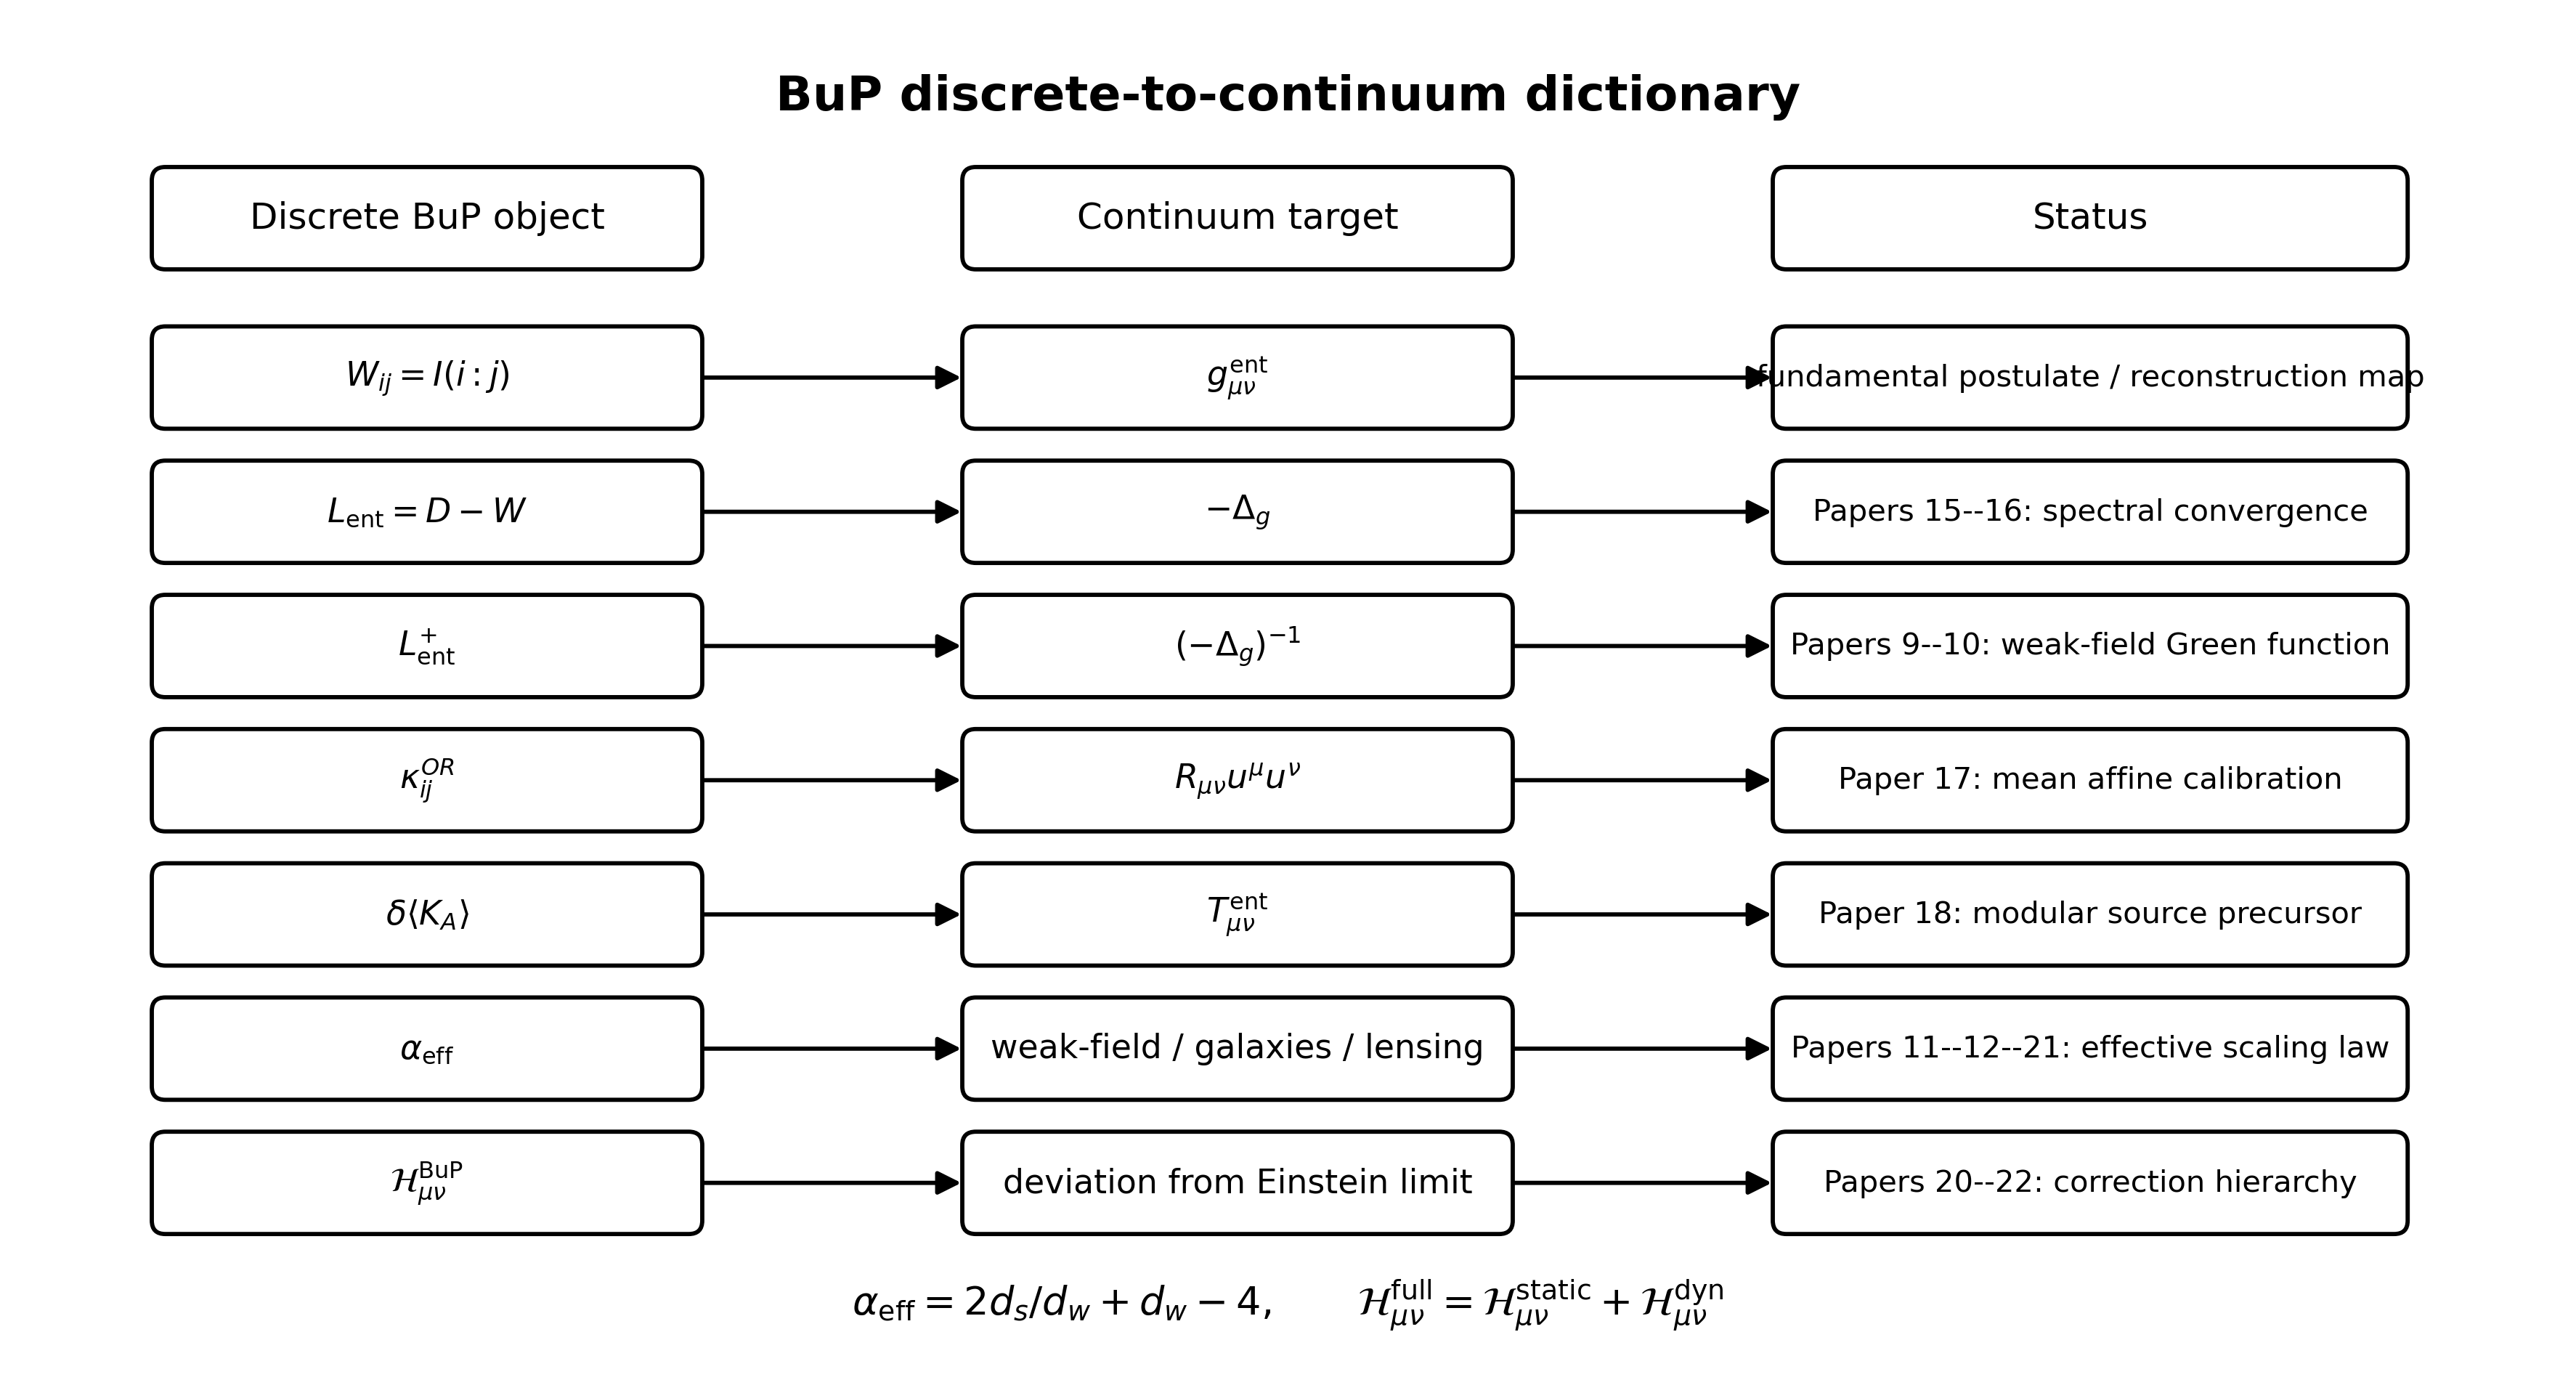
\includegraphics[width=\textwidth]{figures/fig02_discrete_to_continuum_dictionary.png}
\caption{
Discrete-to-continuum dictionary of BuP. The table summarizes the main mappings
from graph quantities to continuum geometric, source and correction objects.
The current status ranges from postulates and controlled numerical convergence
to calibrated proxies and phenomenological sectors.
}
\label{fig:discrete-continuum-dictionary}
\end{figure}

\section{Discrete weak-field limit and entanglement Green function}

Papers 8, 9 and 10 develop the weak-field sector of BuP. Paper 8 constructs a
candidate emergent matter source from local entanglement excitations:
\begin{equation}
  \delta W^{\rm loc}\to S_{\rm flux}.
\end{equation}

The source used in Paper 9 is
\begin{equation}
  S_{\rm flux}
  =
  T_{00}
  -
  \frac12 T_{aa}
  +
  \frac12 T_{\rm grad}
  +
  \|T_{0a}\|.
\end{equation}

Paper 9 then solves the discrete Poisson equation
\begin{equation}
  L_{\rm ent}\Phi_{\rm BuP}=S_{\rm flux}.
  \label{eq:discrete_poisson}
\end{equation}
Equivalently,
\begin{equation}
  \Phi_{\rm BuP}=L_{\rm ent}^{+}S_{\rm flux},
\end{equation}
where \(L_{\rm ent}^{+}\) is the Moore--Penrose pseudoinverse of the
entanglement Laplacian.

This identifies
\begin{equation}
  \boxed{
  G_{ij}^{\rm ent}=(L_{\rm ent}^{+})_{ij}
  }
\end{equation}
as a natural candidate for the discrete gravitational Green function of BuP.

For the best tested regime,
\begin{equation}
  N=20,\qquad \lambda=0.57,\qquad k=5,\qquad \sigma=0.15,
\end{equation}
Paper 9 found
\begin{equation}
  \rho_{\rm Spearman}(S_{\rm flux},|\delta R|)
  =
  0.741,\qquad
  p=1.84\times10^{-4},
\end{equation}
and, after solving Eq.~\eqref{eq:discrete_poisson},
\begin{equation}
  \rho_{\rm Spearman}(\Phi_{\rm BuP},|\delta R|)
  =
  0.738,\qquad
  p=2.01\times10^{-4}.
\end{equation}

Thus the propagated potential retains almost all of the geometric information
contained in the source. Together with the spectral convergence of Paper 16,
\begin{equation}
  L_{\rm ent}\to-\Delta_g,
\end{equation}
this supports the weak-field limit
\begin{equation}
  L_{\rm ent}^{+}\to(-\Delta_g)^{-1}.
\end{equation}

\section{Effective propagator law}

Paper 11 identifies the effective radial law of the BuP propagator:
\begin{equation}
  \boxed{
  \alpha_{\rm eff}
  =
  \frac{2d_s}{d_w}
  +
  d_w
  -
  4.
  }
  \label{eq:alpha_eff}
\end{equation}
Here \(d_s\) is the spectral dimension, \(d_w\) is the walk dimension, and
\(\alpha_{\rm eff}\) controls the effective power law of the gravitational
propagator.

The Newtonian fixed point is
\begin{equation}
  \alpha_{\rm eff}=1.
\end{equation}
For the diffusive value \(d_w=2\), one obtains \(d_s=3\). Therefore ordinary
Newtonian behavior corresponds to the fixed point
\begin{equation}
  \boxed{(d_s,d_w)=(3,2).}
\end{equation}

\section{Cosmological dimensional sector}

Papers 2, 3 and 4 develop the cosmological branch of BuP. The key idea is that
the effective background dimension can vary with redshift:
\begin{equation}
  d(z)=D_C-\frac{\Delta d}{1+X(z)^\alpha}.
\end{equation}
The gravitational coupling is modified through
\begin{equation}
  \boxed{
  G_{\rm eff}(z)=\frac{2}{d(z)-1}G.
  }
\end{equation}

Paper 2 obtained a cosmological fit with
\begin{equation}
  \sigma_8=0.772,
\end{equation}
\begin{equation}
  D_C=3.0598,
  \qquad
  H_0=63.67,
  \qquad
  \Omega_m=0.3448,
\end{equation}
and
\begin{equation}
  \Delta AIC=-6.23,
  \qquad
  \Delta BIC=-3.71.
\end{equation}

Paper 3 confirmed that the same dimensional mechanism reduces the
\(\sigma_8\) tension relative to \(\Lambda\)CDM:
\begin{equation}
  \sigma_8^{\rm BuP}=0.772,
  \qquad
  \sigma_8^{\Lambda{\rm CDM}}\simeq0.811.
\end{equation}

Paper 4 adds a local density-dependent dimensional correction:
\begin{equation}
  d(z,\delta)=d_{\rm bg}(z)-\varepsilon\delta.
\end{equation}
The comparison gives
\begin{equation}
  \varepsilon_{\rm JWST}=0.0113,
  \qquad
  \varepsilon_{\rm micro}(N=20)=0.0065.
\end{equation}

Thus the cosmological branch is naturally assigned to the dimensional
correction sector \(\mathcal H_{\mu\nu}^{\rm dim}\).

\section{Galactic sector and SPARC}

Papers 12, 13 and 14 apply the propagator law to galaxies. Paper 12 uses the
chain
\begin{equation}
  \Sigma(R)
  \to
  (d_s(r),d_w(r))
  \to
  \alpha_{\rm eff}(r)
  \to
  V(r).
\end{equation}
The core law remains Eq.~\eqref{eq:alpha_eff}, now with radius-dependent
dimensions:
\begin{equation}
  \alpha_{\rm eff}(r)
  =
  \frac{2d_s(r)}{d_w(r)}
  +
  d_w(r)
  -
  4.
\end{equation}

Paper 12 showed that this mechanism can reproduce individual SPARC rotation
curves. A representative result is
\begin{equation}
  \chi^2_{\rm red}({\rm NGC3198})=0.994.
\end{equation}

Paper 13 closes the microscopic bridge:
\begin{equation}
  |\Psi\rangle
  \to
  I_{ij}
  \to
  \rho_{\rm ent}(R)
  \to
  \Sigma(R).
\end{equation}
Its central message is:
\begin{equation}
  \boxed{
  \text{Matter encodes entanglement; entanglement reconstructs matter.}
  }
\end{equation}

Paper 14 provides the publication-grade SPARC comparison. Its constrained
full-sample run over 175 galaxies gives
\begin{equation}
  {\rm median}\ \chi^2_{\rm red,BuP}=0.467,
\end{equation}
\begin{equation}
  {\rm median}\ \chi^2_{\rm red,NFW2p}=1.332,
\end{equation}
with BuP better than NFW2p on \(146/175\) galaxies, i.e. \(83.4\%\).

\section{Spectral continuum limit}

Papers 15 and 16 establish the spectral geometry side of the Einstein limit.
The target is
\begin{equation}
  c_NL_N\to-\Delta_g.
\end{equation}

Paper 16 tests the low spectrum of the graph Laplacian against the
Laplace--Beltrami spectrum on controlled geometries. For the circle,
\begin{equation}
  \text{mean relative spectral error}=0.0051.
\end{equation}
For the flat torus,
\begin{equation}
  \text{mean relative spectral error}=0.0266.
\end{equation}
This supports the identification \(L_{\rm ent}\to-\Delta_g\).

The spectral action \(\mathrm{Tr}\,L_{\rm ent}^{-\beta}\) then admits a
heat-kernel interpretation:
\begin{equation}
  \mathrm{Tr}(e^{-t\Delta_g})
  \sim
  (4\pi t)^{-D/2}
  \left(
  a_0+a_1t+a_2t^2+\cdots
  \right).
\end{equation}
The \(a_1\) term contains the scalar curvature contribution, while higher
coefficients generate higher-curvature corrections.

\section{Discrete Ricci curvature limit}

Paper 17 studies the Ricci curvature side of the Einstein limit. The central
relation is
\begin{equation}
  \frac{\kappa^{OR}}{\epsilon}
  \simeq
  B_N+C_NR_{\mu\nu}u^\mu u^\nu.
\end{equation}
At \(N=512\), Paper 17 obtained
\begin{equation}
  B_N=-0.301281,
  \qquad
  C_N=0.391933,
  \qquad
  A_N=\frac{1}{C_N}=2.551455.
\end{equation}
Thus the calibrated Ollivier--Ricci estimator is
\begin{equation}
  \widehat R_{OR}
  =
  2.551455
  \left(
  \frac{\kappa^{OR}}{\epsilon}
  +
  0.301281
  \right).
\end{equation}

This is currently a mean-level calibrated Ricci proxy rather than a complete
pointwise convergence theorem. Its role is to support the chain
\begin{equation}
  \kappa^{OR}\to R_{\mu\nu}u^\mu u^\nu.
\end{equation}

\section{Modular source sector}

Paper 18 develops the source side of the Einstein limit. The key identity is
the graph modular first law:
\begin{equation}
  \delta S_A^{\rm graph}
  \simeq
  \delta\langle K_A^{\rm graph}\rangle.
\end{equation}

The graph density matrix proxy is
\begin{equation}
  \rho_A
  =
  \frac{(L_A+\mu I)^{-1}}
  {\mathrm{Tr}(L_A+\mu I)^{-1}},
\end{equation}
with
\begin{equation}
  S_A=-\mathrm{Tr}(\rho_A\log\rho_A),
  \qquad
  K_A=-\log\rho_A.
\end{equation}

Paper 18 found, on the flat torus,
\begin{equation}
  \delta S_A
  =
  -0.000068
  +
  0.989481\,\delta\langle K_A\rangle,
\end{equation}
with \(R^2=0.996590\). On the sphere,
\begin{equation}
  \delta S_A
  =
  -0.000081
  +
  0.989718\,\delta\langle K_A\rangle,
\end{equation}
with \(R^2=0.996592\).

The modular source also predicts localized curvature response:
\begin{equation}
  R^2(|\delta K|,\langle|\Delta\kappa|\rangle_{\rm near})
  =
  0.967229
\end{equation}
on the flat torus, and \(0.982252\) on the sphere. Thus
\(\delta\langle K_A\rangle\) acts as a scalar modular precursor of the emergent
stress-energy tensor. The present limitation is that a full tensor
\(T_{\mu\nu}^{\rm ent}\) is not yet constructed.

\section{Effective Einstein equation}

Paper 19 assembles the three continuum arrows:
\begin{equation}
  L_N\to\Delta_g,
\end{equation}
\begin{equation}
  \kappa^{OR}\to R_{\mu\nu}u^\mu u^\nu,
\end{equation}
and
\begin{equation}
  \delta W_{\rm loc}
  \to
  \delta S_A
  \simeq
  \delta\langle K_A\rangle
  \to
  T_{\mu\nu}^{\rm ent}.
\end{equation}

The target equation is
\begin{equation}
  \boxed{
  G_{\mu\nu}[g^{\rm ent}]
  +
  \Lambda_{\rm ent}g_{\mu\nu}^{\rm ent}
  =
  8\pi G_{\rm eff}T_{\mu\nu}^{\rm ent}
  +
  \mathcal H_{\mu\nu}^{\rm BuP}.
  }
\end{equation}
Here
\begin{equation}
  G_{\mu\nu}=R_{\mu\nu}-\frac12Rg_{\mu\nu}.
\end{equation}
In the smooth, local, low-energy limit,
\begin{equation}
  \mathcal H_{\mu\nu}^{\rm BuP}\to0,
\end{equation}
and BuP reduces to the effective Einstein form
\begin{equation}
  G_{\mu\nu}+\Lambda_{\rm ent}g_{\mu\nu}
  =
  8\pi G_{\rm eff}T_{\mu\nu}^{\rm ent}.
\end{equation}

\section{Correction tensor}

Paper 20 studies the deviation tensor \(\mathcal H_{\mu\nu}^{\rm BuP}\). The
static correction hierarchy is
\begin{equation}
\begin{aligned}
  \mathcal H_{\mu\nu}^{\rm static}
  =
  &\ \mathcal H_{\mu\nu}^{\rm spec}
  +
  \mathcal H_{\mu\nu}^{\rm curv}
  +
  \mathcal H_{\mu\nu}^{\rm source} \\
  &+
  \mathcal H_{\mu\nu}^{\rm dim}
  +
  \mathcal H_{\mu\nu}^{\rm nonlocal}
  +
  \mathcal H_{\mu\nu}^{\rm topo}
  +
  \mathcal H_{\mu\nu}^{\rm finite}.
\end{aligned}
\label{eq:static_H}
\end{equation}

Paper 22 adds the dynamical sector \(\mathcal H_{\mu\nu}^{\rm dyn}\). Therefore,
\begin{equation}
  \boxed{
  \mathcal H_{\mu\nu}^{\rm full}
  =
  \mathcal H_{\mu\nu}^{\rm static}
  +
  \mathcal H_{\mu\nu}^{\rm dyn}.
  }
\end{equation}

Paper 20 clarifies that the current \(H_{\rm dim}\) and \(H_{\rm nonlocal}\)
quantities are phenomenological proxies, not homogeneous tensor norms. A future
goal is therefore to define a common norm such as
\begin{equation}
  \|\mathcal H^{(a)}\|
  =
  \frac{
  \left(
  \int d^Dx\sqrt g\,
  \mathcal H^{(a)}_{\mu\nu}
  \mathcal H^{(a)\mu\nu}
  \right)^{1/2}
  }{
  \left(
  \int d^Dx\sqrt g\,
  G_{\mu\nu}G^{\mu\nu}
  \right)^{1/2}
  }.
\end{equation}

% --- FIGURE 3 : Hiérarchie du tenseur de correction ----------------------------
\begin{figure}[htbp]
\centering
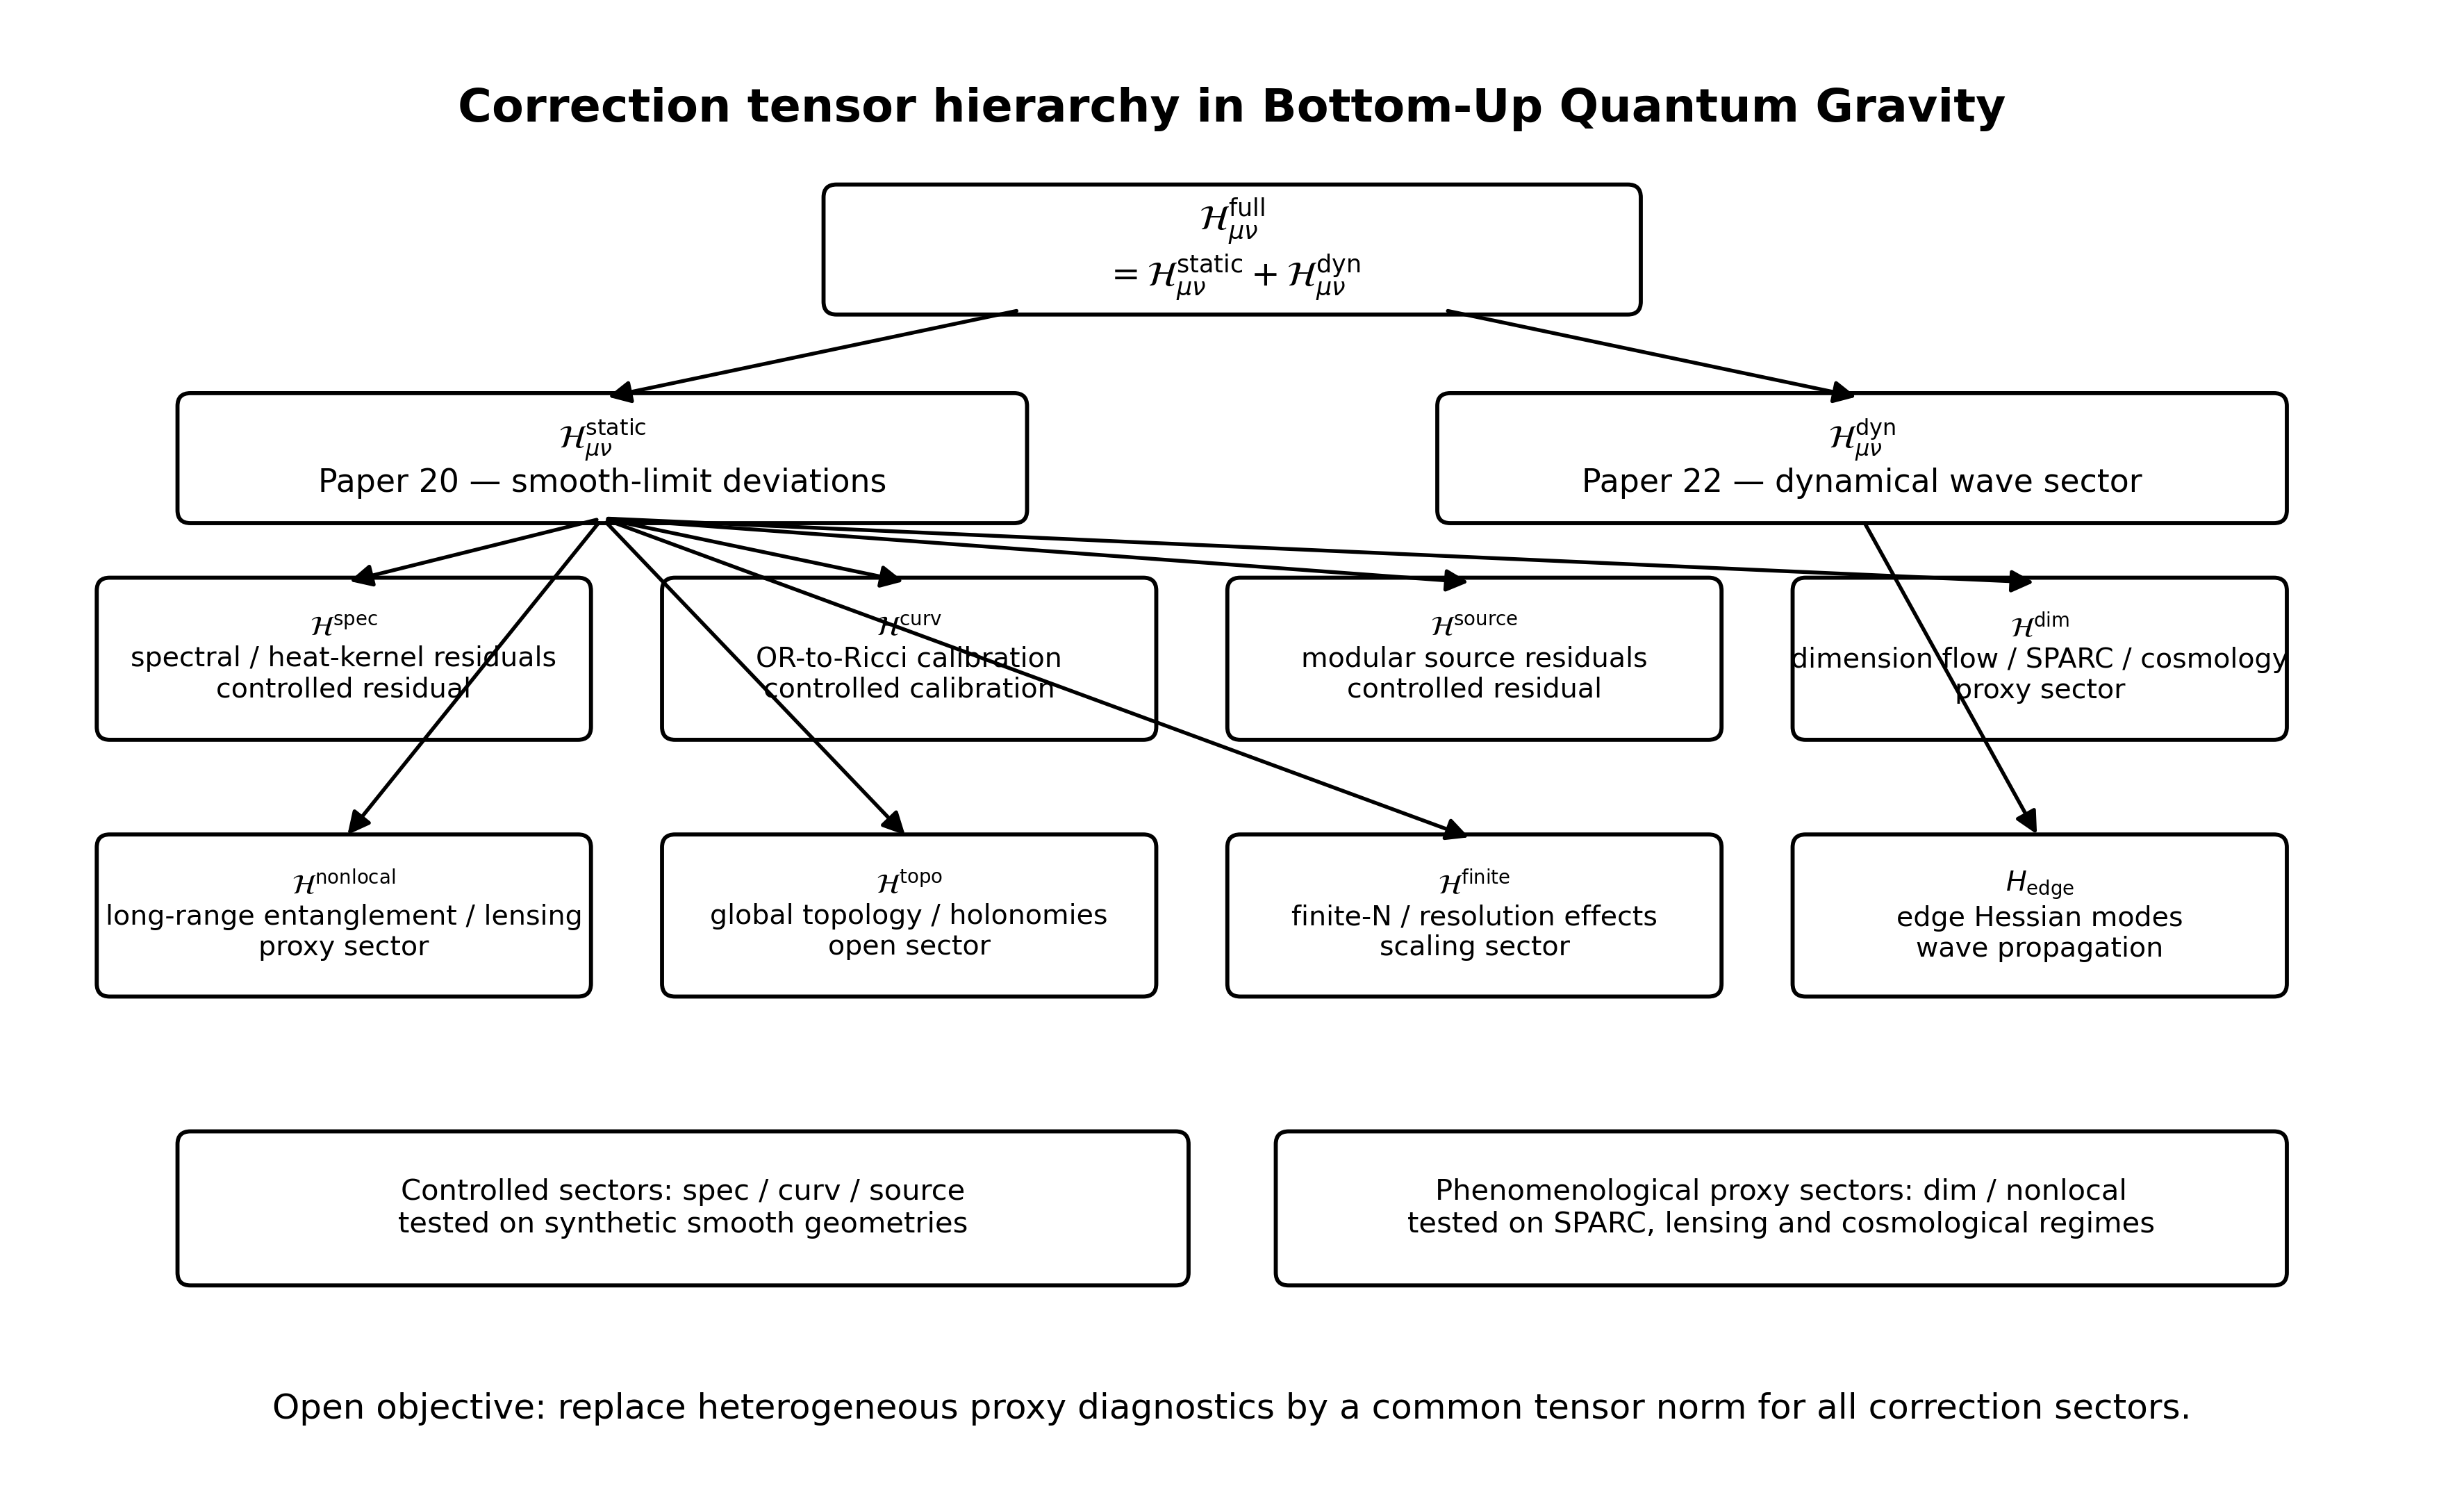
\includegraphics[width=\textwidth]{figures/fig03_correction_tensor_hierarchy.png}
\caption{
Hierarchy of the BuP correction tensor. Paper 20 defines the static correction
sector, while Paper 22 adds the dynamical wave sector. Controlled residuals
such as spectral, curvature and source corrections are distinguished from
phenomenological proxy sectors such as dimensional and nonlocal corrections.
}
\label{fig:correction-hierarchy}
\end{figure}

\section{SLACS and strong-lensing fixed point}

Paper 21 connects BuP to the SLACS strong-lensing branch. The central result is
the existence of a fixed point around
\begin{equation}
  \log M_\star\simeq11.58-11.60,
\end{equation}
where
\begin{equation}
  \langle\alpha_{\rm eff}\rangle\simeq1.014.
\end{equation}
This connects the lensing branch to the Newtonian fixed point
\begin{equation}
  \alpha_{\rm eff}=1.
\end{equation}
Thus Paper 21 is naturally assigned to the nonlocal/optical sector
\begin{equation}
  \mathcal H_{\mu\nu}^{\rm nonlocal}.
\end{equation}

\section{Gravitational-wave sector}

Paper 22 develops the dynamical tensor sector of BuP. The main chain is
\begin{equation}
  W_{ij}
  \to
  H_{\rm edge}
  \to
  q_n(t)
  \to
  \text{gravitational-wave-like modes}.
\end{equation}
In the true-edge Hessian formulation, Paper 22 found strong source-mode
coupling:
\begin{equation}
  \overline{\mathrm{corr}}(|J_n|,q_n^{\rm peak})
  =
  0.999718.
\end{equation}
Finite-size scans show a stable wave-speed sector with
\begin{equation}
  c_{\rm edge}\simeq1.
\end{equation}

The dynamical correction sector is therefore
\begin{equation}
  \mathcal H_{\mu\nu}^{\rm dyn}.
\end{equation}

Together, Papers 21 and 22 suggest a cross-scale fixed-point structure:
\begin{equation}
  \alpha_{\rm eff}\simeq1,
  \qquad
  m_{\rm eff}^2\simeq0,
  \qquad
  v_g\simeq1.
\end{equation}
This is the natural location for future tests involving solar-system
constraints, GW170817-type propagation constraints, and lensing fixed points.

% --- FIGURE 4 : Points fixes cross-scale ---------------------------------------
\begin{figure}[htbp]
\centering
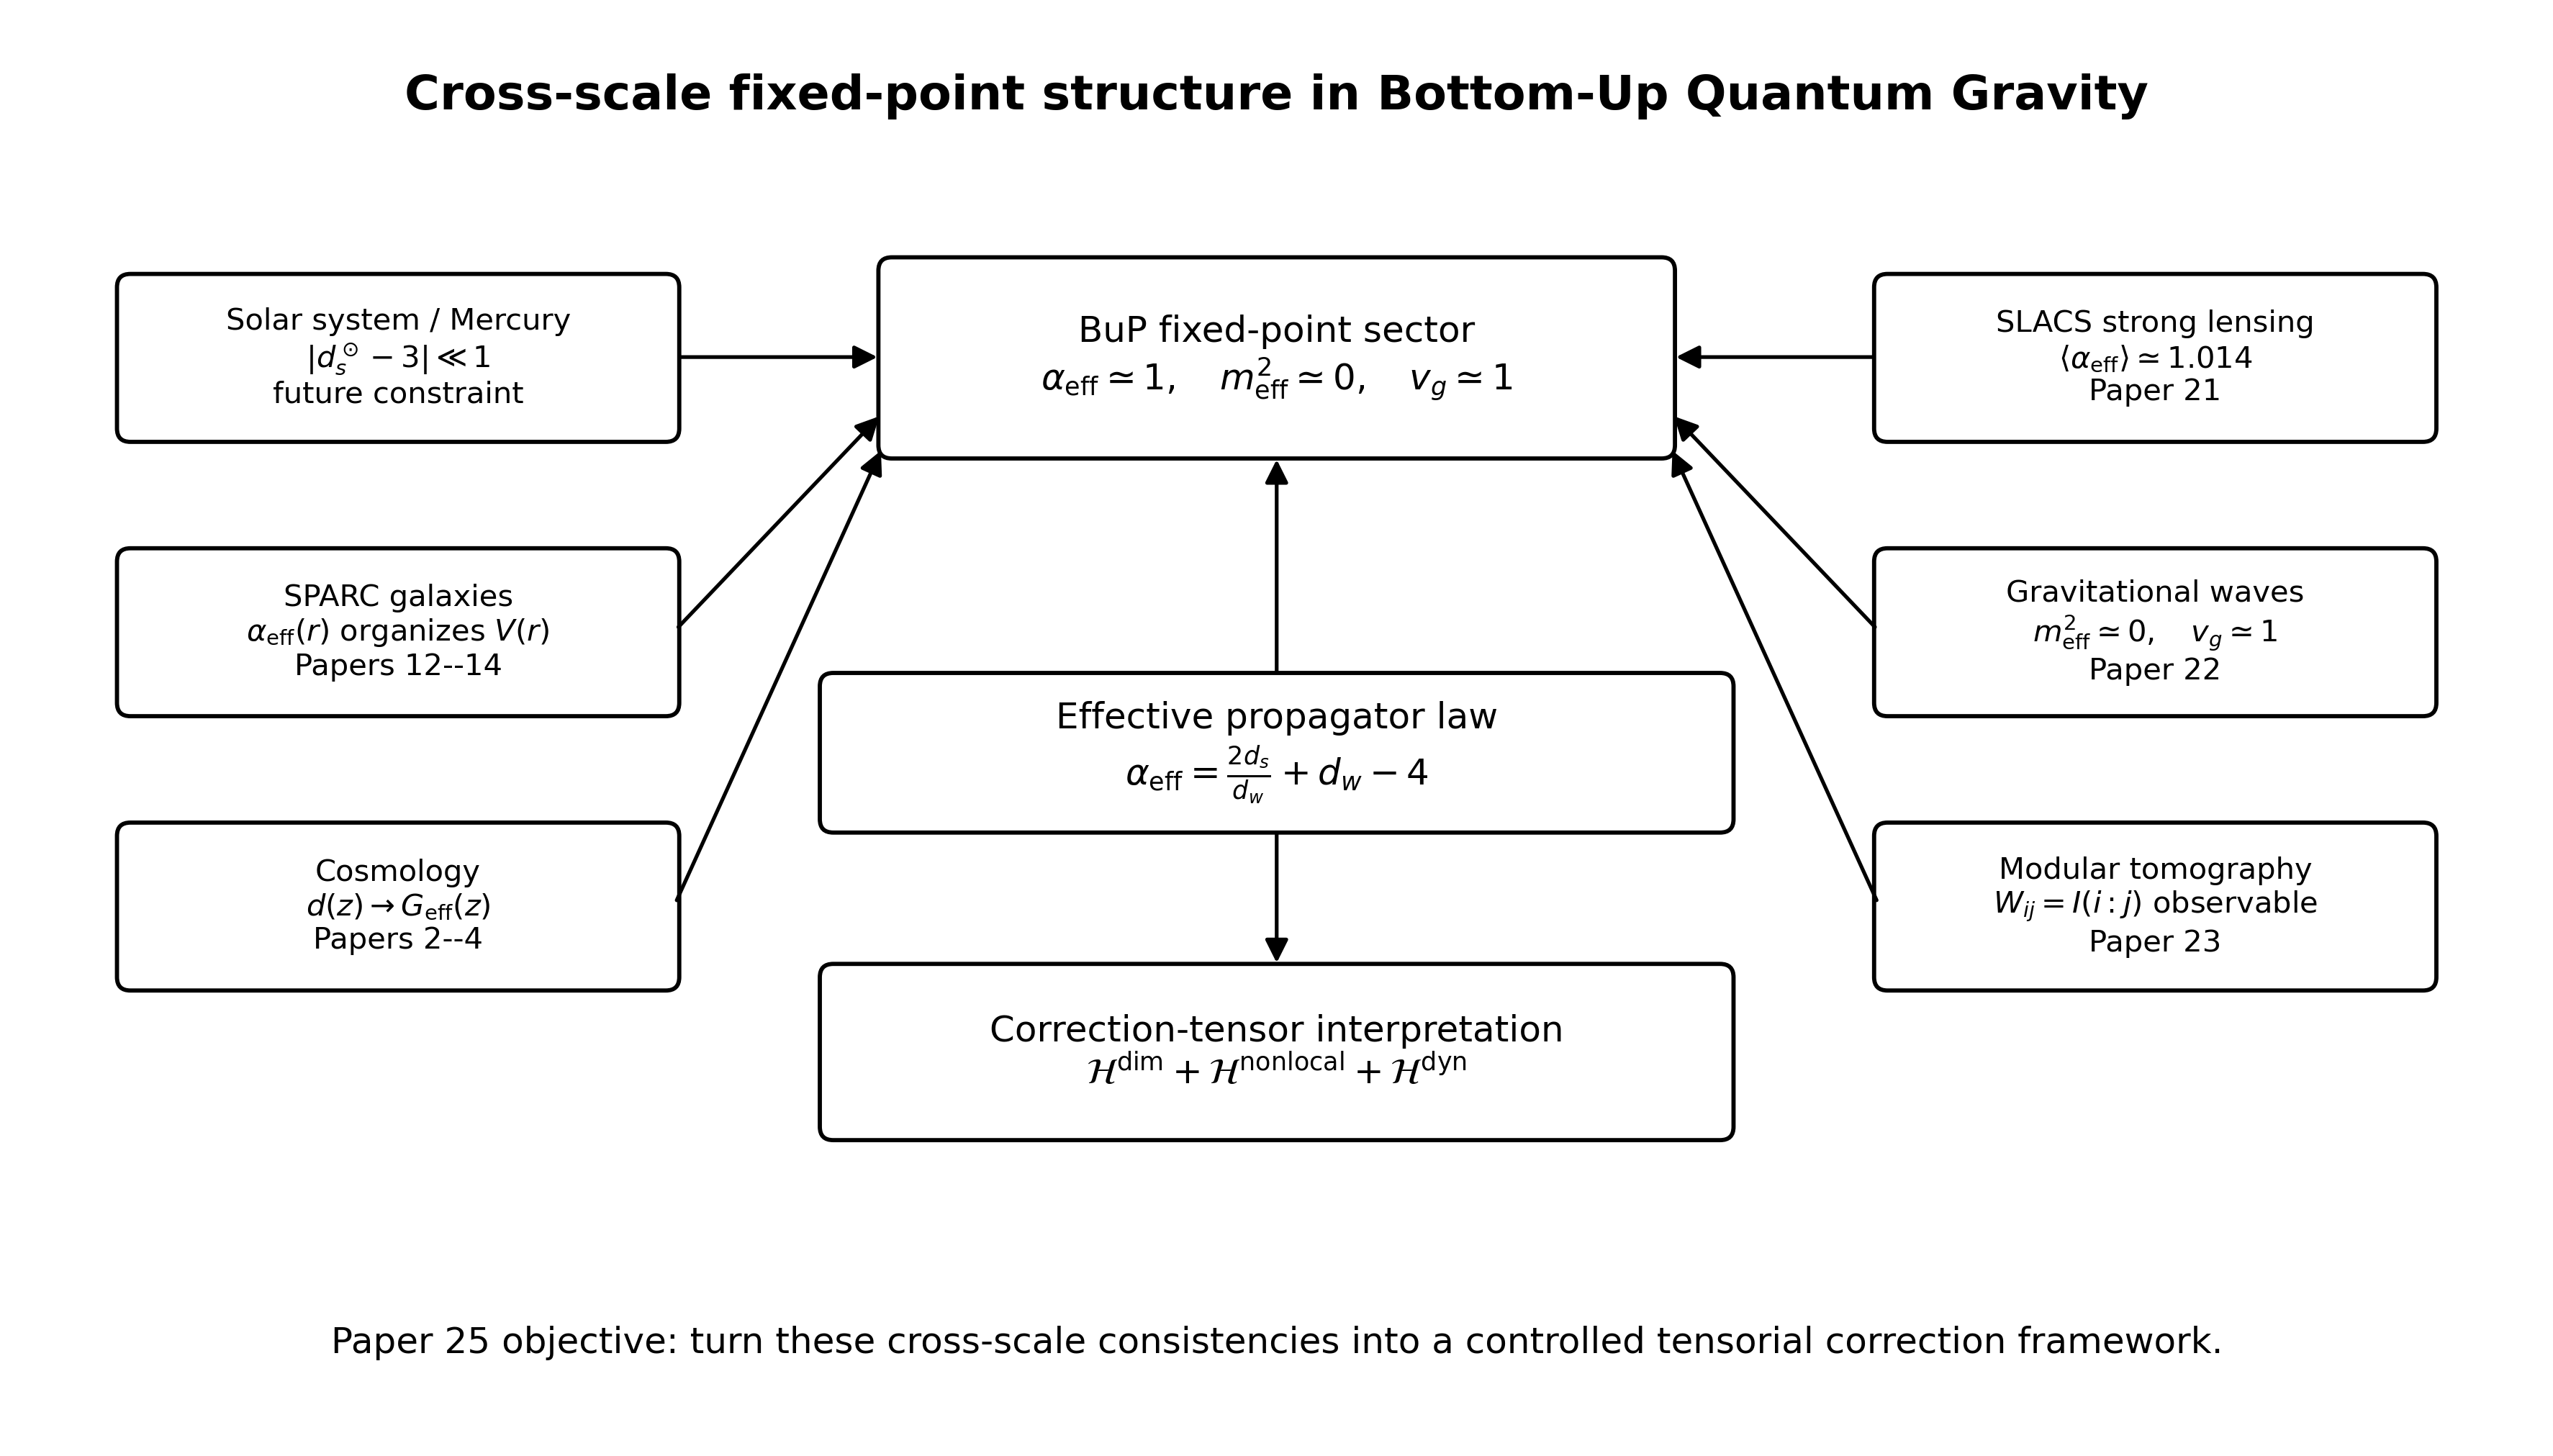
\includegraphics[width=\textwidth]{figures/fig04_cross_scale_fixed_points.png}
\caption{
Cross-scale fixed-point structure in BuP. The effective propagator law
\(\alpha_{\rm eff}=2d_s/d_w+d_w-4\) organizes the Newtonian, galactic, lensing
and cosmological sectors, while Paper 22 adds the dynamical constraints
\(m_{\rm eff}^2\simeq0\) and \(v_g\simeq1\). The objective is to unify these
constraints in the tensorial correction framework.
}
\label{fig:cross-scale-fixed-points}
\end{figure}

\section{Experimental modular tomography}

Paper 23 connects BuP to modular tomography protocols inspired by cold-atom and
quantum-simulator experiments. The key test is whether the entanglement cut
density
\begin{equation}
  \rho_{\rm ent}^{\rm cut}(j)
  =
  \sum_{k\notin A}I(j:k)
\end{equation}
tracks the inverse modular temperature profile
\begin{equation}
  T_{\rm mod}(j)=\frac{1}{\beta_j}.
\end{equation}

This supports the possibility that \(W_{ij}\) is not only a theoretical object,
but a reconstructible experimental observable through mutual-information
tomography.

\section{Target theorem}

The mathematical target of Paper 25 can be stated as follows.

\paragraph{Target theorem.}
Let \((W_N,\rho_N)\) be a sequence of finite entanglement graphs satisfying
\begin{equation}
  W_{ij}\ge0,\qquad W_{ij}=W_{ji},\qquad W_{ii}=0.
\end{equation}
Let \(L_N=D_N-W_N\). Assume that there exists a compact smooth manifold
\((M,g)\), a scale \(\epsilon_N\to0\), and a normalization \(c_N\) such that
\begin{equation}
  c_N\frac{D_N-W_N}{\epsilon_N}\to-\Delta_g
\end{equation}
in a spectral, heat-kernel, or quadratic-form sense.

Assume also that the calibrated Ollivier--Ricci curvature satisfies
\begin{equation}
  \frac{\kappa_N^{OR}}{\epsilon_N}
  =
  B_N+C_NR_{\mu\nu}u^\mu u^\nu+o(1),
\end{equation}
and that local entanglement perturbations satisfy a modular first law,
\begin{equation}
  \delta S_A^{(N)}
  =
  \delta\langle K_A^{(N)}\rangle
  +
  o(1).
\end{equation}

Then the target statement is that the discrete equilibrium equation
\begin{equation}
  \frac{\delta S_{\rm BuP}[W_N,\rho_N]}{\delta W_{ij}}=0
\end{equation}
admits a smooth local continuum limit of the form
\begin{equation}
  G_{\mu\nu}[g^{\rm ent}]
  +
  \Lambda_{\rm ent}g_{\mu\nu}^{\rm ent}
  =
  8\pi G_{\rm eff}T_{\mu\nu}^{\rm ent}
  +
  \mathcal H_{\mu\nu}^{\rm BuP},
\end{equation}
with
\begin{equation}
  \mathcal H_{\mu\nu}^{\rm BuP}\to0
\end{equation}
in the smooth, local, low-energy and large-\(N\) limit.

This is not claimed here as a proven theorem. It is the theorem target
supported by the numerical and phenomenological chain of Papers 2--23.

\section{Open mathematical debts}

\subsection{Derivation of \(c_N\)}

The normalization in \(c_NL_N\to-\Delta_g\) must be derived analytically as a
function of dimension, density, graph scale and sampling.

\subsection{Tensor reconstruction from directional Ricci}

Paper 17 currently supports \(\kappa^{OR}\to R_{\mu\nu}u^\mu u^\nu\). A full
derivation requires reconstructing \(R_{\mu\nu}\) and then
\begin{equation}
  G_{\mu\nu}=R_{\mu\nu}-\frac12Rg_{\mu\nu}.
\end{equation}

\subsection{Full stress-energy tensor}

Paper 18 gives a modular scalar source, \(\delta\langle K_A\rangle\), but a
complete construction of \(T_{\mu\nu}^{\rm ent}\) requires inverting relations of
the form
\begin{equation}
  \delta\langle K_A\rangle
  =
  \int_A
  \xi^\mu
  \delta T_{\mu\nu}^{\rm ent}
  d\Sigma^\nu.
\end{equation}

\subsection{Homogeneous correction norm}

Paper 20 separates controlled residuals and phenomenological proxies. A common
tensor norm for all sectors of \(\mathcal H_{\mu\nu}\) is still required.

\subsection{Micro-to-macro closure}

Paper 13 supports
\begin{equation}
  |\Psi\rangle
  \to
  I_{ij}
  \to
  \rho_{\rm ent}(R)
  \to
  \Sigma(R),
\end{equation}
but a general theorem connecting quantum states, mutual-information graphs and
astrophysical matter profiles remains open.

\subsection{Cross-scale constraints}

Future work must unify the fixed-point constraints from
\begin{equation}
  \text{solar system},\qquad
  \text{SPARC},\qquad
  \text{SLACS},\qquad
  \text{GW speed},\qquad
  \text{cosmology}.
\end{equation}
The relevant unifying quantity is expected to be
\begin{equation}
  \alpha_{\rm eff}
  =
  \frac{2d_s}{d_w}
  +
  d_w
  -
  4.
\end{equation}

\section{Conclusion}

Paper 25 reformulates Bottom-Up Quantum Gravity as a variational theory of
entanglement equilibrium. The central variable is the mutual-information graph
\begin{equation}
  W_{ij}=I(i:j).
\end{equation}
From this graph one obtains the entanglement Laplacian, the weak-field Green
function, the effective propagator law, the cosmological dimensional sector,
the galactic sector, the spectral continuum limit, the discrete Ricci limit,
the modular source sector, the effective Einstein equation, and the correction
tensor.

The resulting chain is
\begin{equation}
  W_{ij}
  \to
  L_{\rm ent},\ \kappa^{OR},\ K_A,\ L_{\rm ent}^{+}
  \to
  g_{\mu\nu}^{\rm ent},\ R_{\mu\nu},\ T_{\mu\nu}^{\rm ent},\ \Phi_{\rm BuP}
  \to
  G_{\mu\nu}
  +
  \Lambda g_{\mu\nu}
  =
  8\pi G T_{\mu\nu}
  +
  \mathcal H_{\mu\nu}.
\end{equation}

The present status is therefore:
\begin{equation}
  \boxed{
  \text{BuP has a coherent variational chain toward effective Einstein
  dynamics, but the complete analytical theorem remains open.}
  }
\end{equation}

\begin{thebibliography}{99}

\bibitem{RyuTakayanagi2006}
S. Ryu and T. Takayanagi,
``Holographic derivation of entanglement entropy from the anti-de Sitter
space/conformal field theory correspondence,''
\emph{Physical Review Letters} \textbf{96}, 181602 (2006).

\bibitem{VanRaamsdonk2010}
M. Van Raamsdonk,
``Building up spacetime with quantum entanglement,''
\emph{General Relativity and Gravitation} \textbf{42}, 2323--2329 (2010).

\bibitem{Swingle2009}
B. Swingle,
``Entanglement renormalization and holography,''
arXiv:0905.1317 (2009).

\bibitem{Jacobson2015}
T. Jacobson,
``Entanglement equilibrium and the Einstein equation,''
\emph{Physical Review Letters} \textbf{116}, 201101 (2016).

\bibitem{FaulknerLewkowyczMaldacena2013}
T. Faulkner, A. Lewkowycz and J. Maldacena,
``Quantum corrections to holographic entanglement entropy,''
\emph{Journal of High Energy Physics} \textbf{2013}, 74 (2013).

\bibitem{ChamseddineConnes1996}
A. H. Chamseddine and A. Connes,
``The spectral action principle,''
\emph{Communications in Mathematical Physics} \textbf{186}, 731--750 (1997).

\bibitem{CoifmanLafon2006}
R. R. Coifman and S. Lafon,
``Diffusion maps,''
\emph{Applied and Computational Harmonic Analysis} \textbf{21}, 5--30 (2006).

\bibitem{Ollivier2009}
Y. Ollivier,
``Ricci curvature of Markov chains on metric spaces,''
\emph{Journal of Functional Analysis} \textbf{256}, 810--864 (2009).

\bibitem{KonopkaMarkopoulouSeverini2008}
T. Konopka, F. Markopoulou and S. Severini,
``Quantum graphity: a model of emergent locality,''
\emph{Physical Review D} \textbf{77}, 104029 (2008).

\bibitem{HamdadPaper2}
F. Hamdad,
``BuP Paper 2 --- Background dimension and cosmological sector,''
Bottom-Up Quantum Gravity Program (2026).

\bibitem{HamdadPaper3}
F. Hamdad,
``BuP Paper 3 --- Sigma8 resolution,''
Bottom-Up Quantum Gravity Program (2026).

\bibitem{HamdadPaper4}
F. Hamdad,
``BuP Paper 4 --- JWST local dimension,''
Bottom-Up Quantum Gravity Program (2026).

\bibitem{HamdadPaper5}
F. Hamdad,
``BuP Paper 5 --- Effective Einstein sector,''
Bottom-Up Quantum Gravity Program (2026).

\bibitem{HamdadPaper6}
F. Hamdad,
``BuP Paper 6 --- Pure BuP equation,''
Bottom-Up Quantum Gravity Program (2026).

\bibitem{HamdadPaper7}
F. Hamdad,
``BuP Paper 7 --- Dynamics of BuP excitations,''
Bottom-Up Quantum Gravity Program (2026).

\bibitem{HamdadPaper8}
F. Hamdad,
``BuP Paper 8 --- Emergent matter in BuP,''
Bottom-Up Quantum Gravity Program (2026).

\bibitem{HamdadPaper9}
F. Hamdad,
``BuP Paper 9 --- Gravitational coupling of emergent matter,''
Bottom-Up Quantum Gravity Program (2026).

\bibitem{HamdadPaper10}
F. Hamdad,
``BuP Paper 10 --- Newtonian limit and propagator,''
Bottom-Up Quantum Gravity Program (2026).

\bibitem{HamdadPaper11}
F. Hamdad,
``BuP Paper 11 --- Effective law of the BuP propagator,''
Bottom-Up Quantum Gravity Program (2026).

\bibitem{HamdadPaper12}
F. Hamdad,
``BuP Paper 12 --- SPARC, alpha effective, spectral and walk dimensions,''
Bottom-Up Quantum Gravity Program (2026).

\bibitem{HamdadPaper13}
F. Hamdad,
``BuP Paper 13 --- Microscopic closure of BuP,''
Bottom-Up Quantum Gravity Program (2026).

\bibitem{HamdadPaper14}
F. Hamdad,
``BuP Paper 14 --- Spectral bridge between modular dynamics and emergent gravity,''
Bottom-Up Quantum Gravity Program (2026).

\bibitem{HamdadPaper15}
F. Hamdad,
``BuP Paper 15 --- From entanglement graphs to Einstein equations,''
Bottom-Up Quantum Gravity Program (2026).

\bibitem{HamdadPaper16}
F. Hamdad,
``BuP Paper 16 --- Spectral continuum limit,''
Bottom-Up Quantum Gravity Program (2026).

\bibitem{HamdadPaper17}
F. Hamdad,
``BuP Paper 17 --- Ollivier--Ricci curvature and Ricci limit,''
Bottom-Up Quantum Gravity Program (2026).

\bibitem{HamdadPaper18}
F. Hamdad,
``BuP Paper 18 --- Emergent stress-energy tensor from entanglement,''
Bottom-Up Quantum Gravity Program (2026).

\bibitem{HamdadPaper19}
F. Hamdad,
``BuP Paper 19 --- Effective Einstein equations from entanglement equilibrium,''
Bottom-Up Quantum Gravity Program (2026).

\bibitem{HamdadPaper20}
F. Hamdad,
``BuP Paper 20 --- Corrections, predictions and observable deviations,''
Bottom-Up Quantum Gravity Program (2026).

\bibitem{HamdadPaper21}
F. Hamdad,
``BuP Paper 21 --- SLACS fixed point,''
Bottom-Up Quantum Gravity Program (2026).

\bibitem{HamdadPaper22}
F. Hamdad,
``BuP Paper 22 --- BuP gravitational waves,''
Bottom-Up Quantum Gravity Program (2026).

\bibitem{HamdadPaper23}
F. Hamdad,
``BuP Paper 23 --- Zoller modular tomography and BuP,''
Bottom-Up Quantum Gravity Program (2026).

\end{thebibliography}

\end{document}
